\documentclass{llncs}
\usepackage{listings}
%
\usepackage{amsmath}
\usepackage{amsfonts}
\usepackage[utf8x]{inputenc}
\usepackage{graphicx}
\usepackage[ruled,vlined]{algorithm2e}
\usepackage[hidelinks]{hyperref}
\usepackage{listings}             % Include the listings-package
\usepackage{graphicx}
\usepackage{xcolor}
\usepackage{caption}
\usepackage{subcaption}


\usepackage{tikz}
\usepackage{pgfplots}


\definecolor{uvblue}{RGB}{0,105,170}
\colorlet{uvblue}{uvblue}
\colorlet{uvbluedark}{black!40!uvblue}
\colorlet{uvbluelight}{white!40!uvblue}


\pgfplotsset{
compat=1.14,
plotl/.style={uvbluelight,no marks,ultra thick,samples=500},
plott/.style={uvblue,no marks,ultra thick,samples=500},
plotd/.style={uvbluedark,no marks,ultra thick,samples=500},
%%
plotA/.style={white!10!uvbluelight,ultra thick,mark=otimes*},
plotB/.style={uvbluelight,ultra thick,mark=triangle*},
plotC/.style={uvblue,ultra thick,mark=pentagon*},
plotD/.style={uvbluedark,ultra thick,mark=diamond*},
plotE/.style={black!40!uvbluedark,ultra thick,mark=square*},
%
asdfas/.style={}
}

%commondefs
%\sloppy
%\allowdisplaybreaks[2]
\newcommand{\Binit}{B_{\mathrm{init}}}
\newcommand{\Pbest}{P_{\mathrm{best}}}
\newcommand{\random}{\mathrm{random}}
\newcommand{\freeff}{\mathit{freeff}}
\newcommand{\neededff}{\mathit{neededff}}
%


\newcommand{\TODO}[1][\empty]{\textcolor{red}{TODO}#1}

\title{\ttitle}
\subtitle{183.663 - Deep Learning for Visual Computing}
\date{\today}

\author{
% \vspace{3.5cm}
Abraham Hinteregger (1025914) \and Christof Schmidt (0627958) }
\institute{
    \email{oerpli@outlook.com}
    \email{e0627958@student.tuwien.ac.at}
}

\begin{document}
% !TeX root = ../dlvc.tex
\newcommand{\ttitle}{kNN Classification and Histograms of Oriented Gradients}
\hyphenation{}
\maketitle

\keywords{kNN classifier, grid search, CIFAR10, histograms of oriented gradients}


\begin{abstract}
This report is a summary of the work done for the first assignment of the course ``Deep Learning for Visual Computing'' in the winter term 2016 at the TU Vienna. The task was to implement a simple kNN classifier and tune the parameters with gridsearch on a subset of the CIFAR10 dataset, for both the raw image data and the extracted HOG features
\end{abstract}



\section{Image Classification} %Describe the image classification problem.
Image classification is one of the most basic tasks in visual computing. The goal is to have some decision procedure (an algorithm or a program usually) that is able to assign labels that should correspond to what a human would recognize on the image. The image is usually provided as a matrix of RGB values in some range, e.g. from 0 to 255 (8 bit per colour channel). The challenge is then, to associate concepts such as ``Skyscraper'' or ``Cat'' with this color information even though there exist a multitude of different skyscrapers and cats with varying colours and appearances.

\section{The CIFAR10 Dataset} % Describe the CIFAR10 dataset.
The \bold{CIFAR-10} Dataset is a is one of the well kown benchmark problems for image classification for object recognition. It has 60000 relativly small RBG images (32 $\times$ 32 pixels) from 10 distinct categories, namely \emph{airplane, automobile, bird, cat, deer, dog, frog, horse, ship,} and \emph{truck}. It is a subset of the larger \bold{CIFAR-100} dataset (consisting of 80 million images) and due to it's limited size ideal for smaller scale projects like this homework assingment. It was created in 2009 by Alex Krizhevsky, Vinod Nair, and Geoffrey Hinton\cite{CIFAR10} \cite{Krizhevsky09learningmultiple}. The current best known performance is at 96.53\%, which is near human capabilities \cite{Graham14a}.


\section{Training, Validation and Test Sets} %Describe the purpose of these sets, why they are required, and how you obtained a validation set in case of CIFAR10.
For training a classifier, and testing the resulting model, a given dataset needs to be split into a training and a test set. Usually, around 80\% are used for training, and 20\% for testing. The classiefier is shown the training data including the labels, and the resulting model is then tested using the not yet shown testing data. This way, overfitting is prevented. In some cases, especially for small datasets, cross validation is used, but for image classification, this is usually too much effort. 

If the classifier has hyper-parameters (like the k in the kNN Classifier) there is also a need for a validation set. The performance of different parameter are tested against the validation set, once the parameters are fixed, the final classifier is again tested against the so far unknown test set. The need for an extra set is again to prevent overfitting.

In the \bold{CIFAR-10} Dataset, we are already given a training and a test test. To obtain a validation set, the original training set is split into a training (80\%) and validation (20\%) set. 

\section{kNN Classifiers} %Describe how the kNN classifier works and how it can be used with images, which are not vectors. Explain what hyperparameters are in general and in case of kNN. How does parameter k generally influence the results?
A kNN classifier is a memory based classification method that calculates a distance measure between the query point with unknown class and all samples in the training set. The $k$ samples from the training set that have the least distance to the query point (hence the name k Nearest Neighbor) are chosen and the classifier predicts that the unknown sample has the same class as the majority (with random tie breaker) of the samples in its neigborhood.

The method can be used with any distance measure, for example the $L^p$-norms L1 (Manhattan distance) and L2 (Euclidean distance) are commonly used. These distance  measures work on vectors, therefore images are usually reshaped to vectors (${3 \times x \times y \to 3\cdot x \cdot y \times 1}$, the exact order doesn't matter as long as it's consistant), normalization (scaling and translating to $0$ mean, $1$ standard deviation) is usually not necessary in this case as all features have the same units. 

kNN Classifiers have two hyperparameters -- the distance metric and the size of the neighborhood considered for each query point (the query point corresponds to the position the data vector points in the high dimensional space if it starts from the origin). A hyperparameter is a parameter of the model/classifier that tries to fit the underlying distribution/system (which may have ``normal'' parameters). As the parameters of the underlying system is usually not known it's necessary to find the best combination of hyperparameters to be able to predict the class of query points with the highest possible accurracy. 
\subsection{k - Neighborhood Size}
As the decision boundary gets rougher the smaller the value of $k$ is, it's usually recommended to choose higher values of $k$ as long as the accuracy for the prediction of the validation set does not suffer. This is the case because a higher parameter $k$ corresponds to a more parsimonious model, i.e. a model with less overfitting\footnote{AIC (Akaice information criterion) and BIC (Bayes information criterion) are more formal versions of this rule of thumb for e.g. linear regression models}. The ragged decision boundaries for kNN with $k =1$ correspond to the Voronoi diagram which is also unstable -- a behaviour that is not desired for a classifier as tiny perturbations in the input set could change the prediction for a query point. For this assignment we used values between $1$ and $40$ for $k$. 
\subsection{Distance metric}
%
\begin{minipage}{0.8\textwidth}
Different distance metrics result in different neighborhoods, for example in the figures on the right the Voronoi diagram (corresponding to kNN with $k=1$) of the same set of points was calculated once with L1 and once with L2 norm as distance metric (images from Wikipedia, created by user Balu.ertl).

It's not obvious wether the L1 or the L2 norm is superior for image classification. The best choice of metric may depend on the kind of picture, for example OCR (optical character recognition) for handwritten text benefits from rotation invariance whereas for printed text this is not necessary.

There are so called \textit{invariant metrics} for this kind of tasks that improve the accuracy with kNN classification significantly compared to simple L1/L2 norms by providing additional invariants such as rotational invariance (for example \textit{Transformation Distance}, Simard et al. 1993)
\end{minipage}
%
\begin{minipage}{0.3\textwidth}
\centering

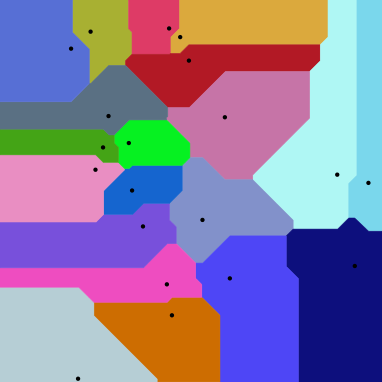
\includegraphics[width=0.57\textwidth]{./img/voroL1.png}
\captionof{figure}{L1 metric}
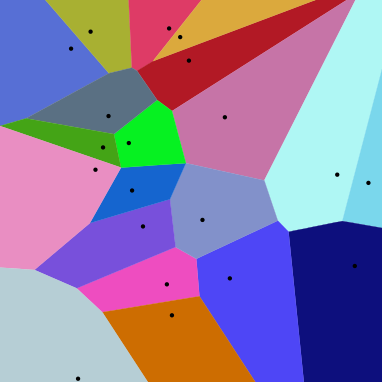
\includegraphics[width=0.57\textwidth]{./img/voroL2.png}
\captionof{figure}{L2 metric}
\end{minipage}

\clearpage
\section{kNN Classification of CIFAR10} %Introduce the tiny version of CIFAR10. Describe what hyperparameter optimization is and why it is important. Explain your search strategy and visualize the results based on the output of knn_classify_tinycifar10.py.
For this assignment, we were allowed to use a subset of the \bold{CIFAR-10} dataset, which is called \emph{TinyCifar10} from now on. For that, we use only 10\% of the dataset for training, validation and testing. This allows to perform the tests in a much shorter timescale. The need for that came from the \emph{hyperparameter optimization} task.
\subsection{Hyperparameter optimization}
The parameter for k and the norms can be choosen arbitrarily. To obtain good results, different values and combinations needs to be tested. This process is called \emph{hyperparameter optimization}. In the lecture, two method were introduced: One is random search, were the parameter are taken at random for a fixed number of attempts. The other, that we implemented, is the grid search, where systematically a range of values is tested (possibly with gaps in between) and the best found combination is chosen. See figure \ref{figparam} for the results.

\begin{figure}[h!t]
\newcommand{\plotref}[1]{{[~\ref{plt:#1}~]}}
\centering
% !TeX root = ../dlvc.tex
\begin{tikzpicture}
\begin{axis}[
	height=300pt
,	xlabel={$k$ Neighborhood size}
,	ylabel={Accuracy (\%)}
,	width=1\textwidth
,	xtick={1,5,...,39}
,	ticks=major
,	xmajorgrids
, 	major grid style={line width=0.1pt,draw=gray!30}
,	ymin=20
,	ymax=42
%,	xmin=1, xmax=37
,	legend pos=south east]
%\addplot[plotA]{sin(x)};
\addplot [plotE]table[x index=0,y index=2, meta index = 0] {./data/a1.txt};\addlegendentry{L1 norm, HOG vector }
\addplot [plotD]table[x index=0,y index=1, meta index = 0] {./data/a1.txt};\addlegendentry{L2 norm, HOG vector }
\addplot [plotC]table[x index=0,y index=4, meta index = 0] {./data/a1.txt};\addlegendentry{L1 norm, raw vector \ \ }
\addplot [plotA]table[x index=0,y index=3, meta index = 0] {./data/a1.txt};\addlegendentry{L2 norm, raw vector \ \ }
\addplot[black!30!red,mark=square,ultra thick,only marks,forget plot]table[x index=0,y index=1, meta index = 0] {./data/a1-test.txt};\label{plt:t1}
\addplot[black!30!red,mark=pentagon*,thick,only marks,forget plot]table[x index=0,y index=2, meta index = 0] {./data/a1-test.txt};\label{plt:t2}
\end{axis}
\end{tikzpicture}

\caption{Accuracy of kNN classification with neighborhood sizes (k) and L1 and L2 norms on raw image and HOG vectors. Classification on HOG consistently outperforms class. on raw data and kNN with L1 norm is superior to kNN with L2 norm. Performance of best parameters ($k=21, \text{L1 norm}$) on test set with raw \plotref{t2} and HOG data \plotref{t1}. }
\label{figparam}

\end{figure}

% !TeX root = ../dlvc.tex
\section{The Importance of Features} %Think about reasons why performing kNN classification directly on the raw images does not work well. Describe what a feature is and why operating on features instead of raw images is beneficial in case of kNN. Briefly explain what HOG features are. Compare the results when using these features (knn_classify_hog_tinycifar10.py) to those obtained using raw images and discuss them. Even with HOG features, the performance is still much lower than that of CNNs (90\% accuracy and more on the whole dataset). Think of reasons for why this is the case.

When comparing the raw images with kNN, the result is how similiar one image is to the other. So even if the same content was shown, but just with different colors, they would appear very different to the kNN. Or a change of the background color, while irrelevant to the object, would have a big impact on the distance. Thus, a comparision of features of an image seems more appropriate for the task given. 

Features are some properties of a given data instance. The can be very simple or rather complex. In the case of images classification we want features that allow us to better identify objects from a raw image. One important feature of an image are the edges, so edge detection is a common method used in feature extraction. 

\subsection{HOG features}
The \emph{Histograms of Oriented Gradients for Human Detection} were introduced in  \cite{Dalal:2005:HOG:1068507.1069007}. It takes images as an input and extracts localized gradient orientations. The initial work was focused on pedestrian recognition, but it works well on identifying other objects as well. It is a process covering several steps, where gradients are computed, divided into local cells, and an histogram is computed. The results are combined and normalized and yield in a much lower dimensional vector than the input image. In our case, the raw image was 3072-dimensional, while the HOG features are only 144-dimensional. 

As seen in fig. \ref{figparam} the HOF features outperform the raw data by more than 10\%, which is no surprise given above reasons. The computation was also a lot faster due to the reduced dimensionality.

But the HOG results are still far behind state-of-the-art methods like CNNs. The reason is, while the CNNs will also extract lower level features like edges and gradients, they can easily overcome problems like occlusion and displacement, because they define higher level feature. They are able to find human-like, or cat-like features by combining the lower lever features. 


%% Ausgelagert ins File dlvc1-6.tex
%\section{The Importance of Features} %Think about reasons why performing kNN classification directly on the raw images does not work well. Describe what a feature is and why operating on features instead of raw images is beneficial in case of kNN. Briefly explain what HOG features are. Compare the results when using these features (knn_classify_hog_tinycifar10.py) to those obtained using raw images and discuss them. Even with HOG features, the performance is still much lower than that of CNNs (90\% accuracy and more on the whole dataset). Think of reasons for why this is the case.

\newpage

\bibliographystyle{unsrt}
\bibliography{references}

\end{document}

\bibliographystyle{splncs}
